% ==================== 2.3.2.3 HCP ====================
\jiegou{2.3.2.3}{六方密堆积结构（HCP）}

以镁为例建立六方密堆积结构模型，建模参数见表~\ref{tab:hcp}。六方晶系以 $a$、$b$ 轴
夹角 $120^\circ$ 为特征，HCP 结构的非对称单元含有两个不等价原子。

\begin{table}[H]
  \centering
  \caption{六方密堆积（HCP）结构的建模参数}
  \label{tab:hcp}
  \begin{tabular}{ll}
    \toprule
    项目 & 参数 \\
    \midrule
    空间群 & $P\,6_3/m\,m\,c$（No.~194） \\
    晶格常数 & $a=b=3.2085$\,\AA，$c=5.2106$\,\AA，$\alpha=\beta=90^\circ$，
      $\gamma=120^\circ$ \\
    原子坐标 & Mg：$(0,0,0)$、$(1/3,2/3,1/2)$（$2c$ 位） \\
    化学式单元数 & $Z=2$ \\
    \bottomrule
  \end{tabular}
\end{table}

\begin{figure}[H]
  \centering
  \subcaptionbox{空间群与晶格常数设置}{%
    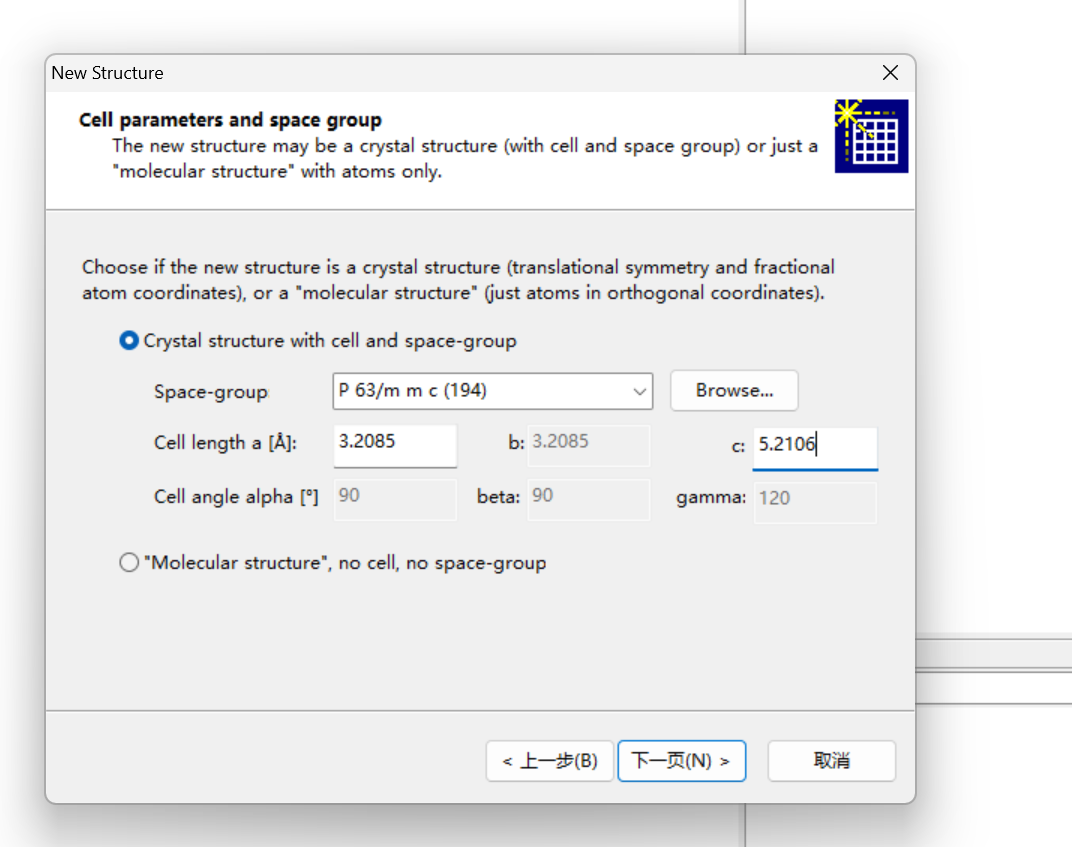
\includegraphics[width=0.44\textwidth]{assets/hcp/a.png}}
  \hfill
  \subcaptionbox{非对称单元原子（Mg）添加}{%
    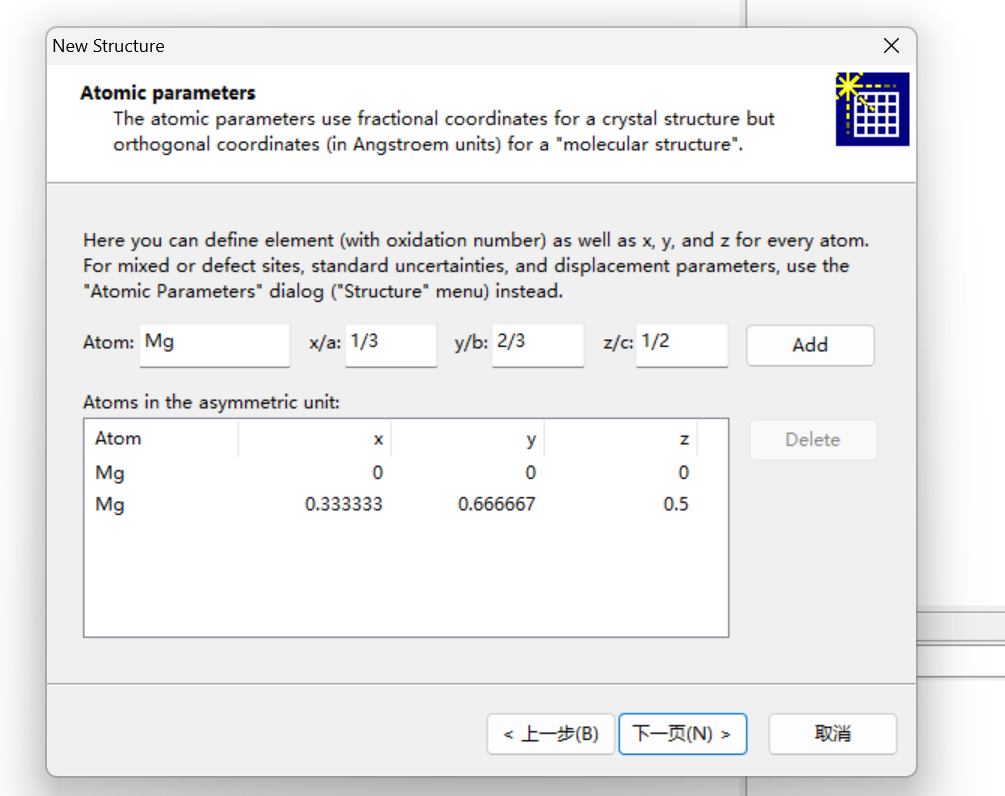
\includegraphics[width=0.44\textwidth]{assets/hcp/b.png}}
  \caption{六方密堆积（HCP）结构的参数设置}
  \label{fig:hcp-param}
\end{figure}

\begin{figure}[H]
  \centering
  \subcaptionbox{结构模型（视角一）}{%
    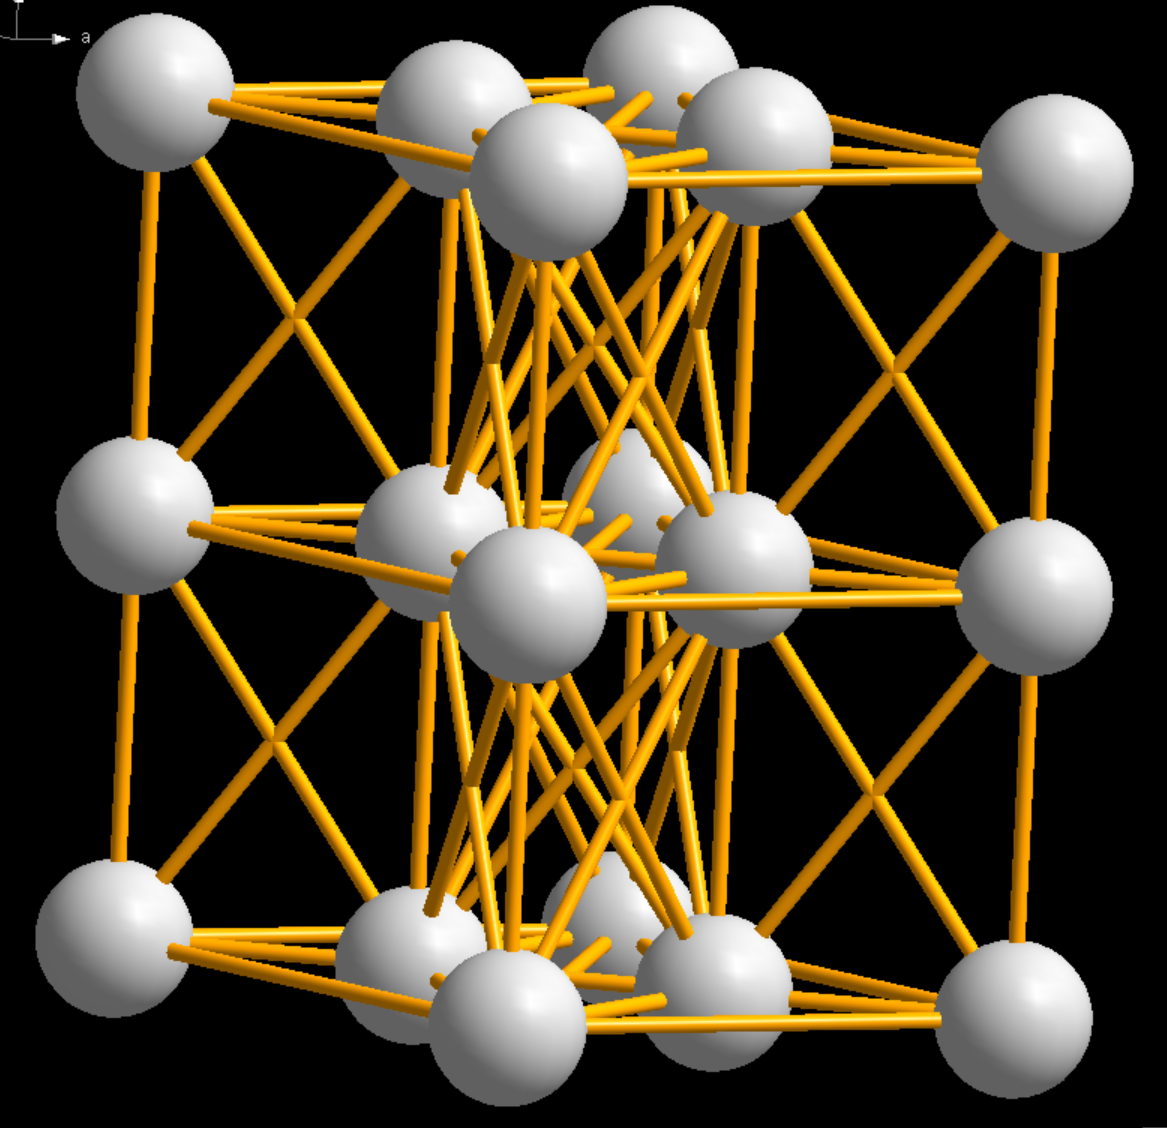
\includegraphics[width=0.44\textwidth]{assets/hcp/c.png}}
  \hfill
  \subcaptionbox{结构模型（视角二）}{%
    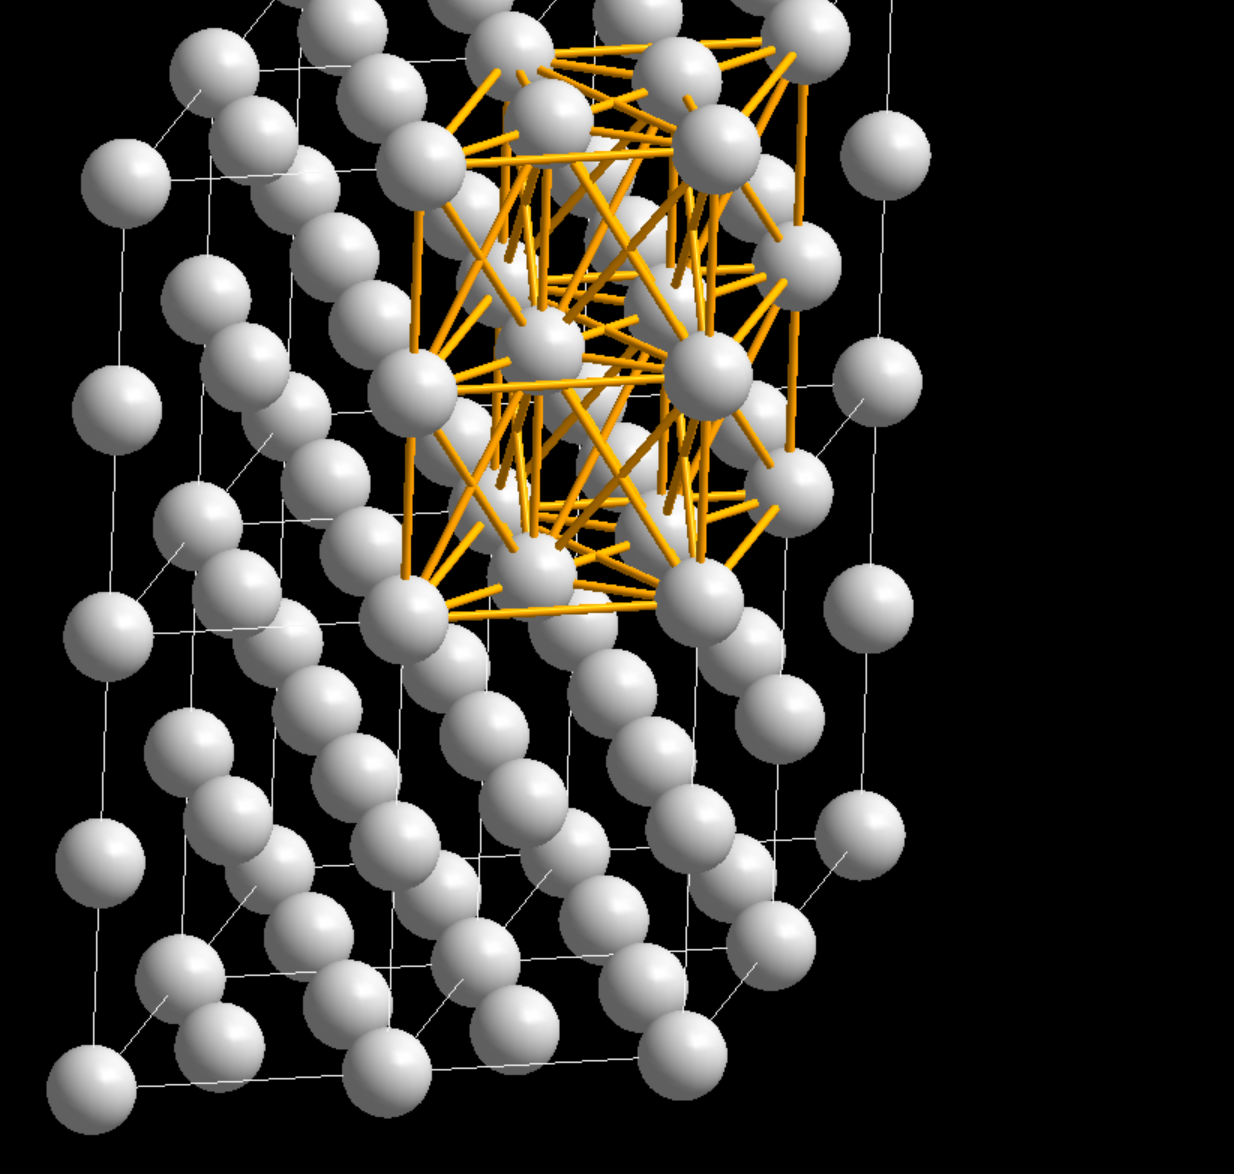
\includegraphics[width=0.44\textwidth]{assets/hcp/extra.png}}
  \caption{六方密堆积（HCP）结构的晶体结构模型}
  \label{fig:hcp-model}
\end{figure}

\begin{figure}[H]
  \centering
  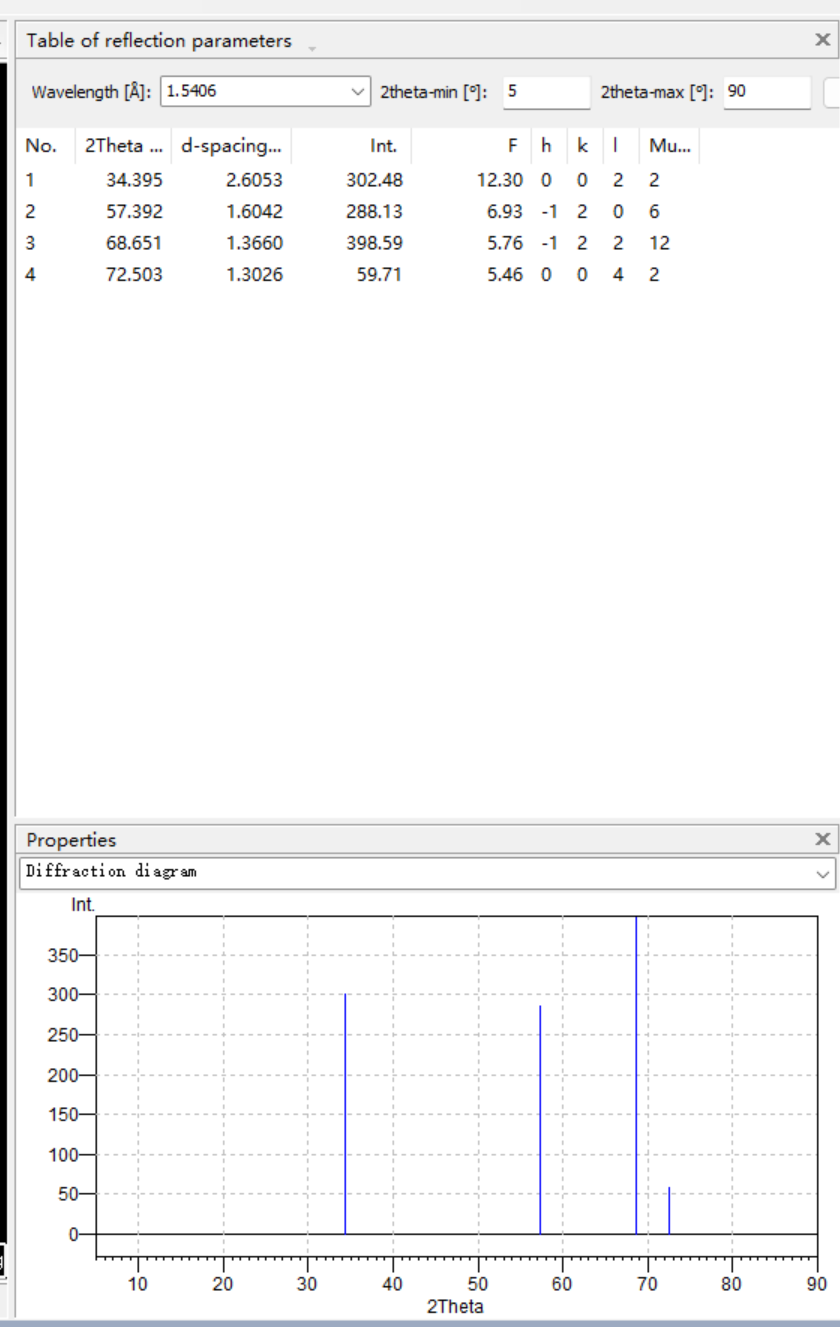
\includegraphics[width=0.4\textwidth]{assets/hcp/d.png}
  \caption{Diamond 模拟的六方密堆积（HCP）结构粉末衍射图}
  \label{fig:hcp-xrd}
\end{figure}

\begin{figure}[H]
  \centering
  \subcaptionbox{$(0001)$ 密排面（基面）视图}{%
    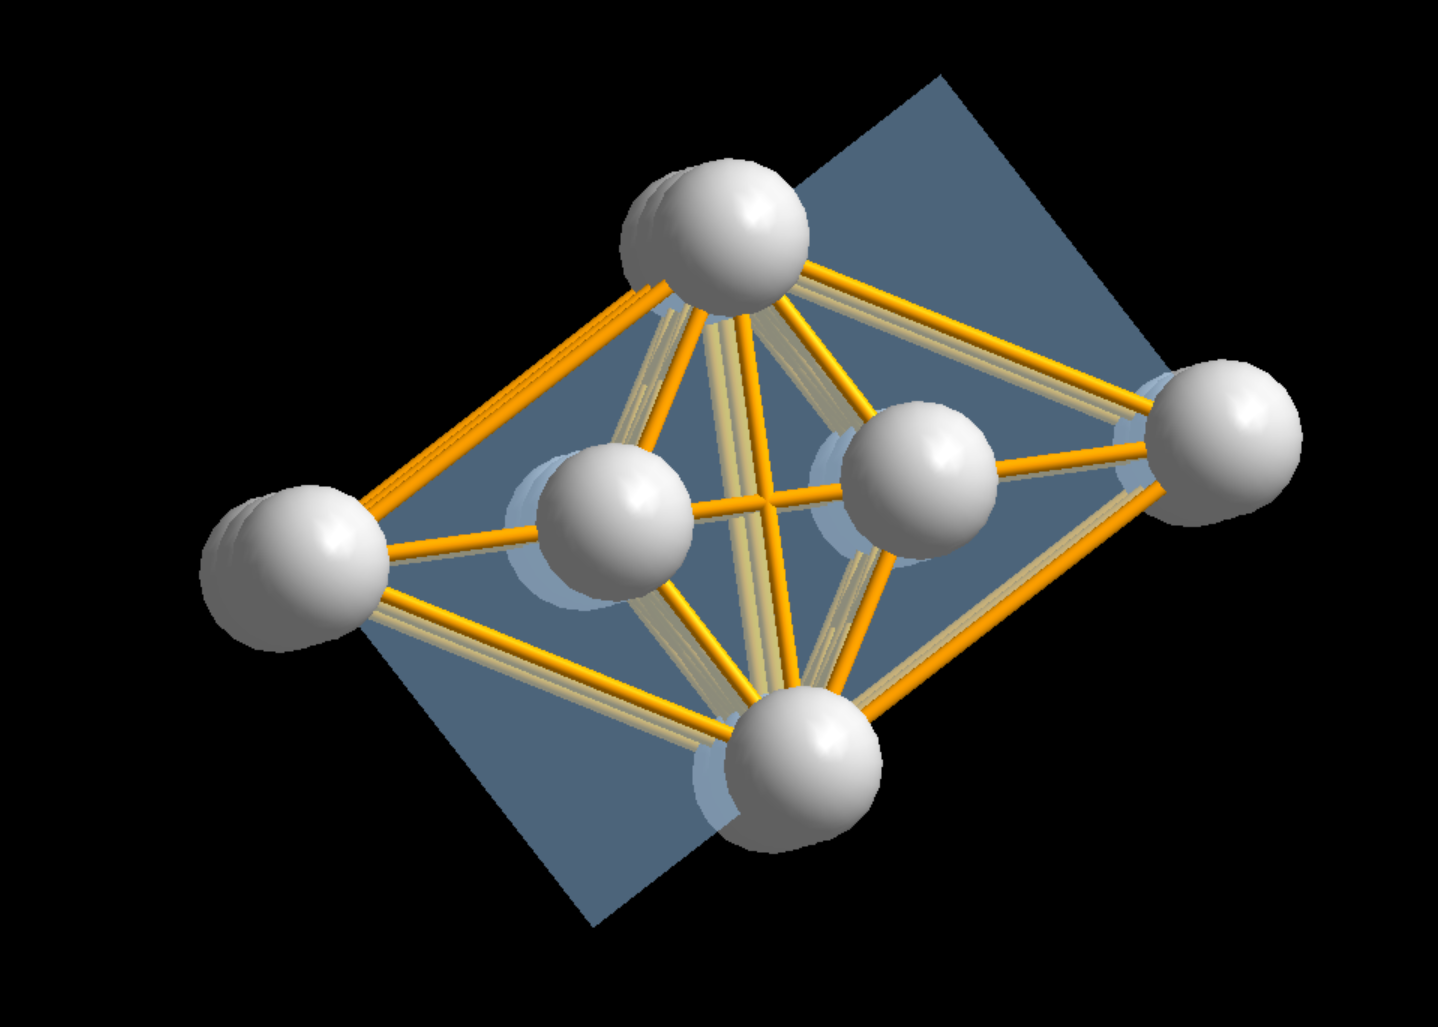
\includegraphics[width=0.46\textwidth]{assets/hcp/e.png}}
  \hfill
  \subcaptionbox{最近邻配位多面体（配位数 12）}{%
    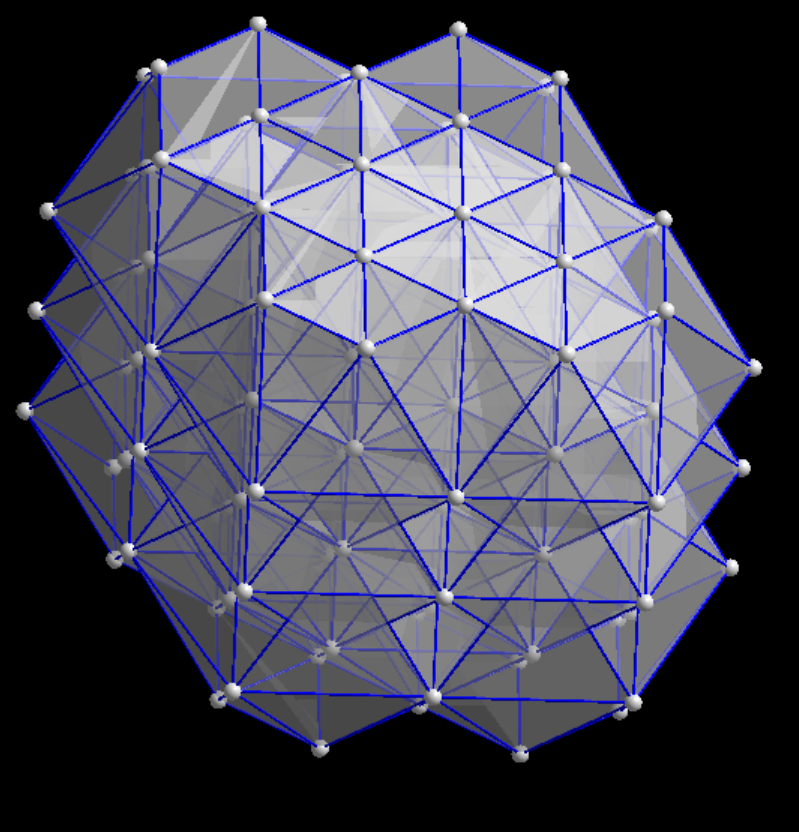
\includegraphics[width=0.44\textwidth]{assets/hcp/f.png}}
  \caption{六方密堆积（HCP）结构的密排面与配位多面体}
  \label{fig:hcp-plane}
\end{figure}

\textbf{结构特征。}HCP 晶胞的两个原子分别位于 $(0,0,0)$ 与 $(1/3,2/3,1/2)$，晶胞内
原子数为 2。与 FCC 一样，HCP 也是原子最紧密堆积方式之一，两者堆积因子相同，但堆积
顺序不同。

\begin{enumerate}[label=（\arabic*）]
  \item \textbf{轴比}：本模型的轴比 $c/a=5.2106/3.2085\approx1.624$，略小于刚球密
    堆积的理想值 $c/a=\sqrt{8/3}\approx1.633$。轴比的偏离意味着层间原子不完全按刚球
    相切排列，实际金属（Mg、Zn 等）的轴比多略偏离理想值。
  \item \textbf{配位数}：每个原子有 12 个最近邻原子（同层 6 个、上下层各 3 个），
    配位多面体为六方密堆积特征的多面体（图~\ref{fig:hcp-plane}(b)）。
  \item \textbf{原子堆积因子}：在刚球模型下 $r=a/2$，晶胞体积
    $V=\dfrac{\sqrt{3}}{2}a^2c$，故
    \begin{equation}
      \eta=\frac{2\times\frac{4}{3}\pi\left(\frac{a}{2}\right)^3}
                {\frac{\sqrt{3}}{2}a^2c}
        =\frac{2\pi a}{3\sqrt{3}c}
    \end{equation}
    代入理想轴比 $c=\sqrt{8/3}\,a$ 得 $\eta=\pi/(3\sqrt{2})\approx0.7405$。
  \item \textbf{密排面与堆积方式}：密排面为 $(0001)$ 基面（图~\ref{fig:hcp-plane}(a)），
    密排层沿 $[0001]$ 方向按 ABAB 方式交替堆积；FCC 则为 ABCABC 堆积。若晶体生长过程
    中某密排层缺失，FCC 的 ABCABC 序被破坏，很容易形成 ABAB 排列，即 HCP 结构，这是
    许多材料中 FCC $\leftrightarrow$ HCP 结构相变的根源。
\end{enumerate}

空间群符号 $P\,6_3/m\,m\,c$ 表明：$P$ 为六方初基点阵，[001] 方向为 $6_3$ 螺旋轴加
镜面，[100] 方向为镜面 $m$，[120] 方向为 $c$ 滑移面。具有 HCP 结构的典型金属有 Mg、
Zn、Ti、Co 等。
